%%
%% Capítulo 4: Figuras, gráficos e tabelas
%%

\mychapter{Experimentos e Resultados}
\label{Cap:ExperimentosResultados}
Neste trabalho foram feitos três experimentos em relação a criação,
de um modelo cinemático para o robô, o primeiro experimento foi o
treinamento de um modelo de rede neural simples, onde o algoritmo
de aprendizado supervisionado deve buscar uma transformação linear,
que mapeia velocidade linear e angular do robô para as velocidades
angulares das rodas sem levar em consideração as equações das rodas,
o segundo experimento é o treinamento de um modelo cujo os parâmetros
são constantes das equações rodas, onde o algoritmo de aprendizado
de máquina deve realizar uma regressão não linear para encontrar
estes parâmetros, por fim é resolvido analaticamente a cinemática
e é comparado os três modelos. Em relação ao controlador, foi implementado
o controlador Frederico e encontrado as constantes do P.I.D empiricamente.


\section{Experimentos com a Cinemática}
Em todos os treinamentos dos modelos
de rede neural artificial foi utilizado o algoritmo de otimização
RMSprop com uma taxa de aprendizado de 0.0001, um momentum $m =0$,
foi utilizado o \textit{Framework pytorch}, para a criação dos
grafos computacionais e treinamento dos modelos, \textit{pytorch}
permite a criação e prototipagem de um modelo de aprendizagem de
máquina na linguagem \textit{Python} ao mesmo tempo que possui
uma versão em C++ e \textit{Rust}, permitindo criar aplicações
bastante performáticas. Para a criação dos modelos, executado o
algoritmo de coleta de dados para obter um conjunto com 10 mil
pontos, durante o treinamento é dividido este conjunto de dados
onde 60\% dos dados é utilizado para treinamento e 40\% é utilizado
apenas para avaliação, ou seja, a rede não possui informação sobre esses
pontos durante o treinamento, nas figuras \ref{fig:error:quadratico:nao:linear} e
\ref{fig:error:quadratico:linear} a linha vermelha representa o erro de
Avaliação, e a linha azul representa o erro durante o treinamento,
a métrica de erro utilizada para o treinamento e avaliação
foi o erro quadrático médio.

\begin{figure}[H]
    \label{fig:error:quadratico:nao:linear}
    \centering
    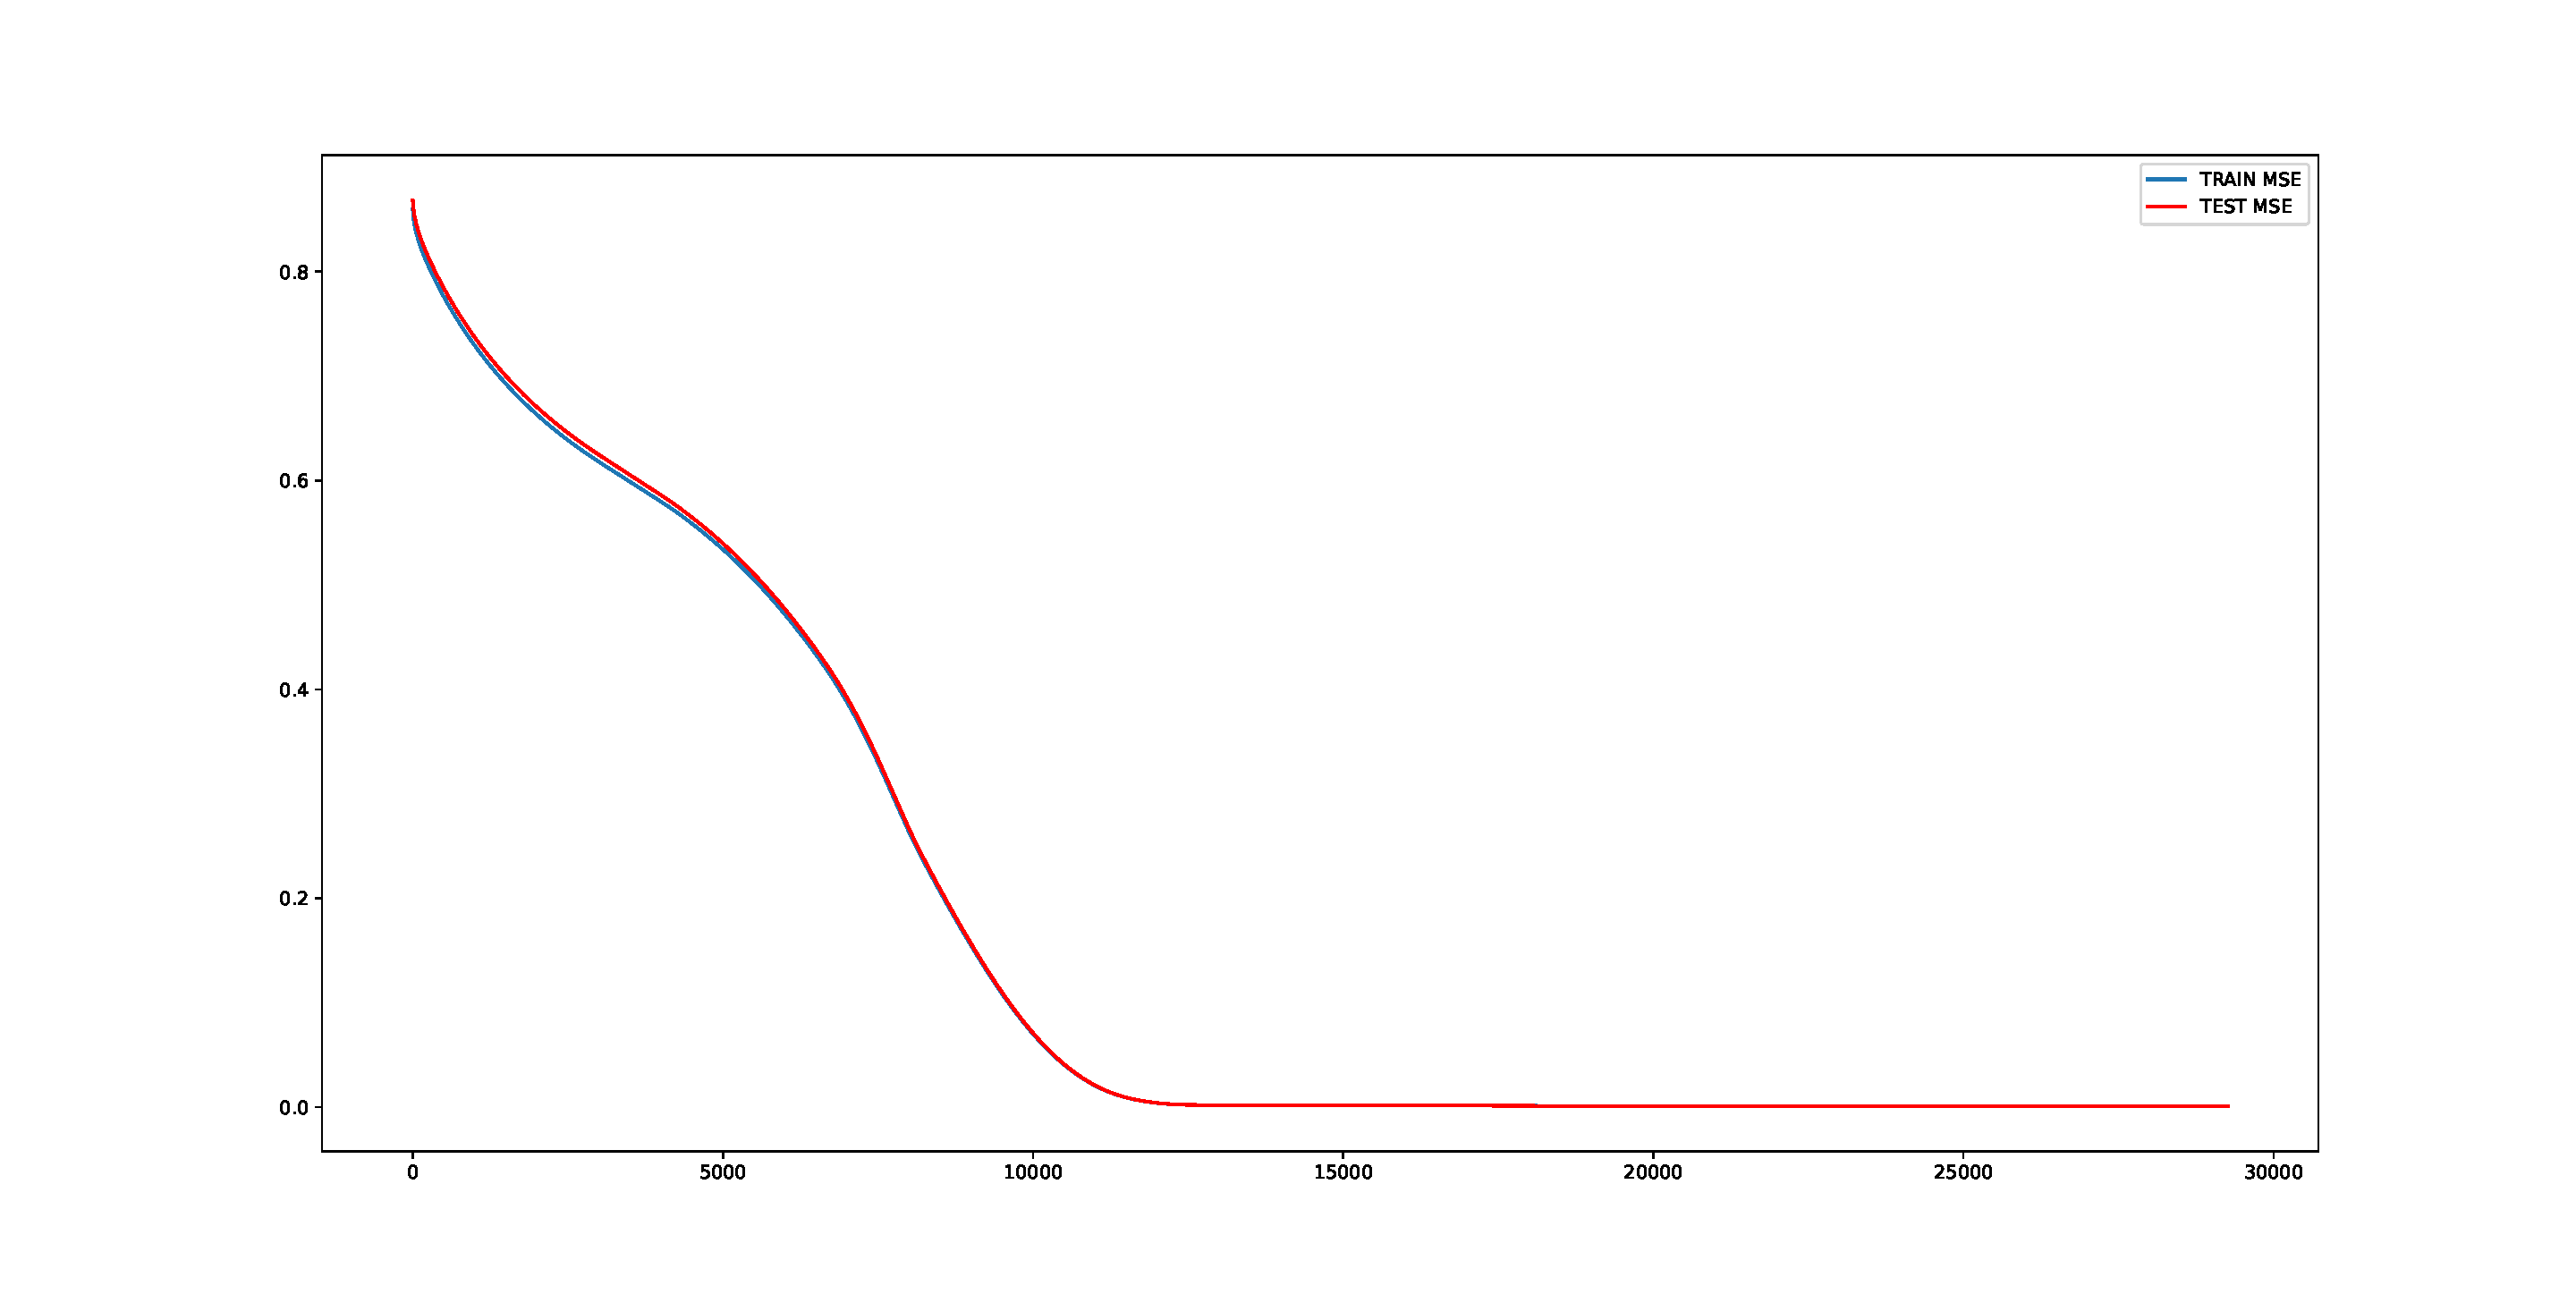
\includegraphics[scale=0.3]{figuras/MSE_error_non_linear.pdf}
    \caption{Erro Médio quadrático regressão não linear}
\end{figure}

\begin{figure}[H]
    \label{fig:error:quadratico:linear}
    \centering
    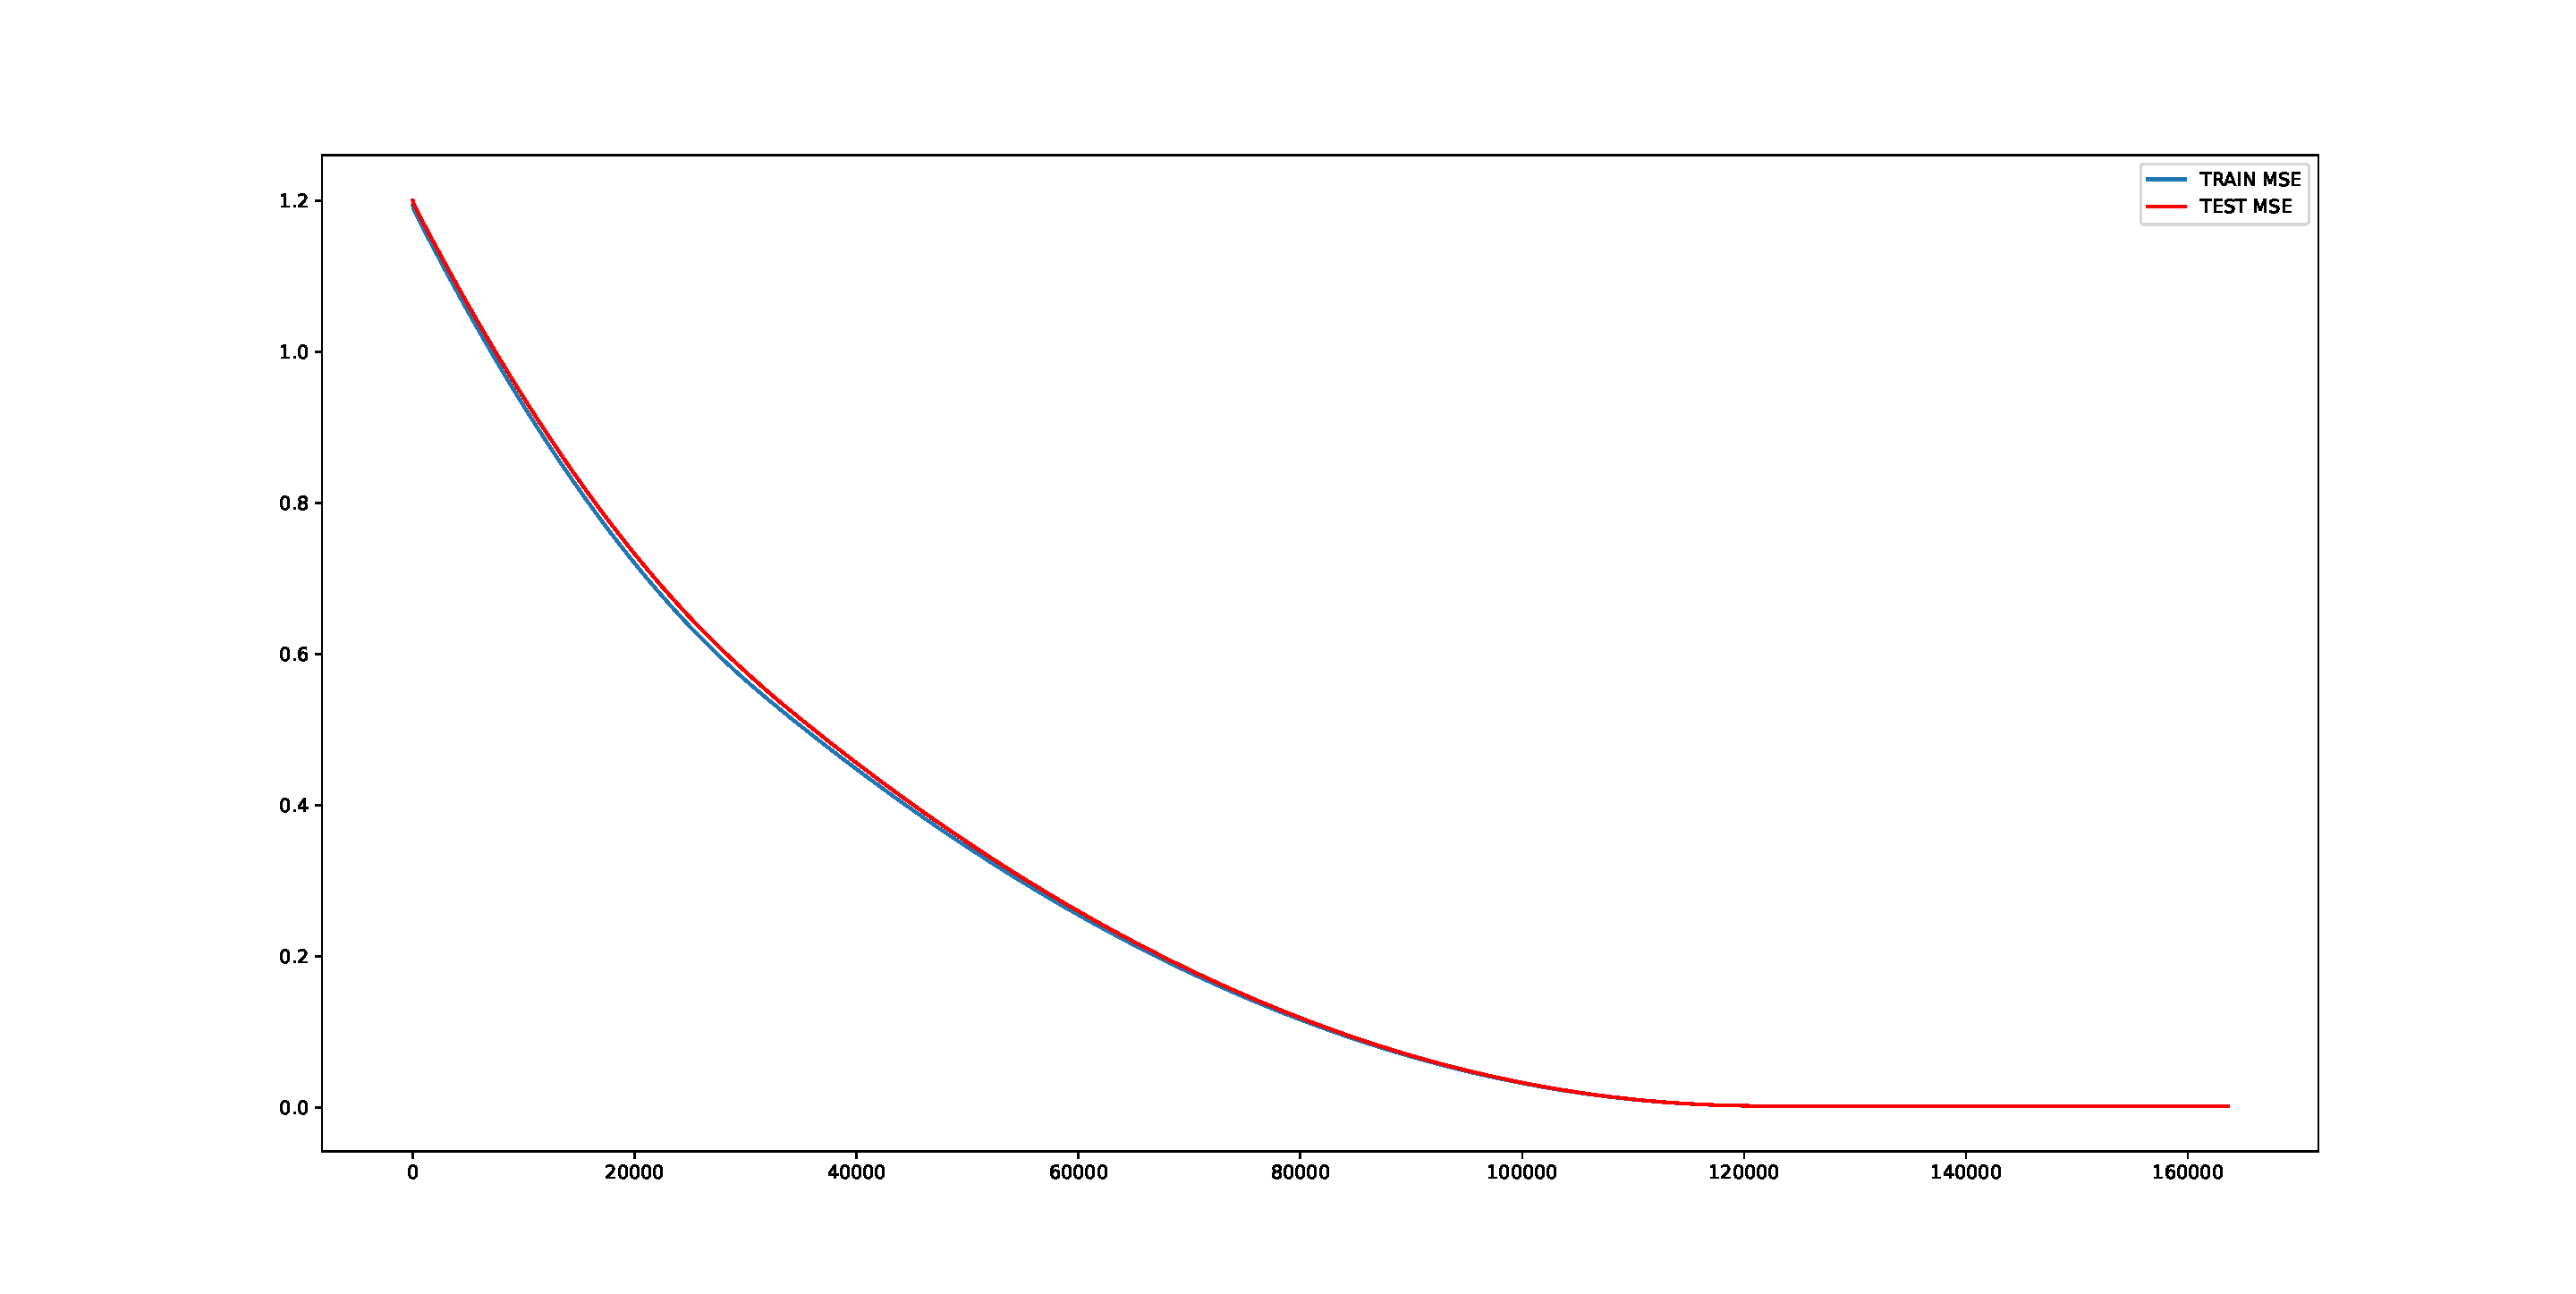
\includegraphics[scale=0.3]{figuras/mse_error_linear.pdf}
    \caption{Erro Médio quadrático regressão linear}
\end{figure}


\begin{table}[H]
    \centering
    \begin{tabular}{c|c}
        \hline
        Erro quadrático médio & modelo \\
        \hline
        0.0013 & modelo regressão linear \\
        \hline
        0.0006 & modelo regressão não linear \\
        \hline
    \end{tabular}
    \caption{Avaliação dos modelos}
\end{table}